\chapter{Výběr bezdrátové technologie pro senzorovou síť}
\label{Výběr bezdrátové technologie pro senzorovou síť}
Tato kapitola porovnává dostupné bezdrátové technologie vhodné pro tento vybraný případ senzorové sítě a na závěr vysvětluje která technologie byla nakonec vybrána a z jakých důvodů.


%%%%%%%%%%%%%%%%%%%%%%%%%%%%%%%%%%%%%%%%%%%%%%%%%%%%%%%%%
\section{Hlavní kritéria pro výběr bezdrátové technologie}
% Mezi hlavní požadavky na navrženou senzorovou síť implementovanou do infrastruktury přístupového systému patří jednoduchost napojení.
% Pro tento vybraný případ se konkrétně jedná o infrastrukturu již zavedeného přístupového systému v budovách několika podniků.
Navržená senzorová síť má být připojena do infrastruktury přístupového systému, který je již zaveden v několika budovách. Jejím účelem je bezdrátové měření veličin např. teplota, vlhkost, CO\textsubscript{2}, pomocí koncových zařízení sítě, která vydrží několik let napájena z baterie při periodě měření několik minut rozmístěných v budově a jejím okolí.
Pro jednoduchost implementace vybraná bezdrátová technologie tedy musí používat pouze bezlicenční pásmo ISM a musí umožňovat implementaci celé sítě bez závislosti na síti třetích stran. 
Dosah by tedy měl být pro pokrytí celé budovy a jejího okolí, ale je zde i možnost napojení více gatewayí rozmístěných po budově k dosažení požadovaného dosahu.
Níže jsou vypsány hlavní kritéria pro výběr bezdrátové technologie pro tuto senzorovou síť.

\begin{itemize}
  \item Nízká cena HW
  \item Jednoduché přípojení koncových zařízení třetích stran (Third party)
  \item Velký počet dostupných koncových zařízení třetích stran na trhu 
  \item Jednoduchá implementace
  \item Nízká spotřeba energie koncových zařízení
\end{itemize}

%%%%%%%%%%%%%%%%%%%%%%%%%%%%%%%%%%%%%%%%%%%%%%%%%%%%%
\section{Kandidátní bezdrátové technologie}
V této sekci jsou rozebrány dostupné bezdrátové technologie, které jsou běžně používány pro bezdrátové měření zařízeními napájenými z baterie a vyhovují stanoveným kritériím vypsaných výše.

\subsection{IQRF}
IQRF je technologie podporována IQRF aliancí \cite{iqrf_alliance}, která je jediným výrobcem IQRF transceiveru \cite{iqrf_transceivers} za cenu v rozsahu \$15-20 za kus a k tomu poskytuje nástroje jako je SDK (Software Development Kit) \cite{iqrf_sdk} a IDE (Integrated Development Environment) \cite{iqrf_ide}.
Technologie IQRF bývá použita k realizaci sítí o topologii typu mesh nebo hvězdice.
Jedna síť má jednoho koordinátora, který slouží jako gateway a může obsahovat až 240 zařízení (včetně koordinátora). Pro požadavek vyššího počtu zařízení je efektivnější zřetězit více sítí, s jednotlivými koordinátory a různými RF kanály pro vyšší propustnost.
% https://iqrf.org/support/networkingfaq
Dosah na přímou viditelnost je až 500 m a velikost datového obsahu (dále v práci uvedeno jako payload) jednoho paketu může být až 64 B \cite{iqrf_rf}.
% Z hlediska kriérií pro tento vybraný případ je u této technologie nevýhodou nízký počet zařízení třetích stran dostupných na trhu. 
Většinou je tato technologie použita pro realizaci uživatelské sítě, kde gateway je použita jedna z dostupných od IQRF aliance a koncová zařízení sítě jsou vytvořena vývojáři s použitím transceiverů od IQRF aliance
\cite{paper_iqrf}.



\subsection{Wireless M-Bus}
Wireless M-Bus (Meter-Bus) je standard specifikovaný v evropské normě EN 13757 \cite{EN 13757}, popisující fyzickou, síťovou a aplikační vrstvu, původně navržen pro aplikace bezdrátového měření jako rozšíření průmyslové datové sběrnice M-Bus \cite{wirelessMBus_automatizace}.
Po několika letech v průmyslu bezdrátových měřících systémů se tato technologie rozšířila do oblasti průmyslu senzorových sítí.
Komunikace koncových zařízení je rozdělena do několika módů v závislosti na orientaci komunikace a objemu vysílaných dat \cite{wirelessMBus01}, \cite{wirelessMBus02}. 
Wireless M-Bus síť má hvězdicovou topologii o dosahu 500 m v pásmu 868 MHz.
Komunikaci vždy zahajuje koncové zařízení, které koncentrátor obsluhuje \cite{wirelessMBus03}, \cite{wirelessMBus04}.
Transceivery vyrábí více různých firem za cenu okolo \$25-30 za kus.


\subsection{LoRa}
LoRa (Long Range) je modulace navržena firmou Semtech.
LoRaWAN je otevřený standardizovaný síťový protokol a systémová architektura navržen LoRa Aliancí definovný v LoRaWAN specifikaci \cite{lorawan_specification} vytvářející MAC (media acess control) vrstvu nad fyzickou vrstvou LoRa se zabezpečením přenášených dat. 
%The LoRaWAN nodes communicate directly with the LoRaWAN gateway \cite{Internet of Things (IoT) using LoRa technology}.
Síť má hvězdicovou topologii, kde komunikaci zahajuje koncové zařízení a koncentrátor ho obsluhuje \cite{LoRa Network Architecture: LoRaWAN}.
Pro nízkou spotřebu protokol umožňuje ladit SF (Spreading Factor) odpovídající přenosové rychlosti, pro regulaci dosahu, který je až 15-22 km mimo městskou část a 3-8 km ve městské části \cite{lorawan_specification}.
V některých oblastech některé firmy poskytují pokrytí LoRaWAN sítí a proto je tato technologie velmi populární. Na trhu je mnoho koncových zařízení i gatewayí s jejichž vzájemnou kompatibilitou není problém. Gateway přeposílá přijaté pakety s daty z koncových zařízení na server, kde je payload zpracován na základě dokumentace od výrobce daného koncového zařízení.
Semtech je jediným výrobcem integrovaných obvodů podporujících LoRa modulaci. Na trhu je dostupných mnoho transceiverů, které používají tento integrovaný obvod, některé dokonce obsahují implementovaný LoRaWAN protokol.
Transceiver pro gateway má cenu okolo \$130 a umožňuje současně přijímat pakety od koncových zařízení na více kanálech a přenosových rychlostech. Je zde i možnost udělat jednokanálovou gateway, která je schopna přijímat v jednu chvíli pouze na jednom kanále a jedné přenosové rychlosti s použitím transceiveru pro koncová zařízení za cenu okolo \$5-20. V takové sítí pak musí být všechna koncová zařízení nakonfigurována na jednu konkrétní frekvenci a přenosovou rychlost.

% \begin{figure}[!h]
%     \centering
%     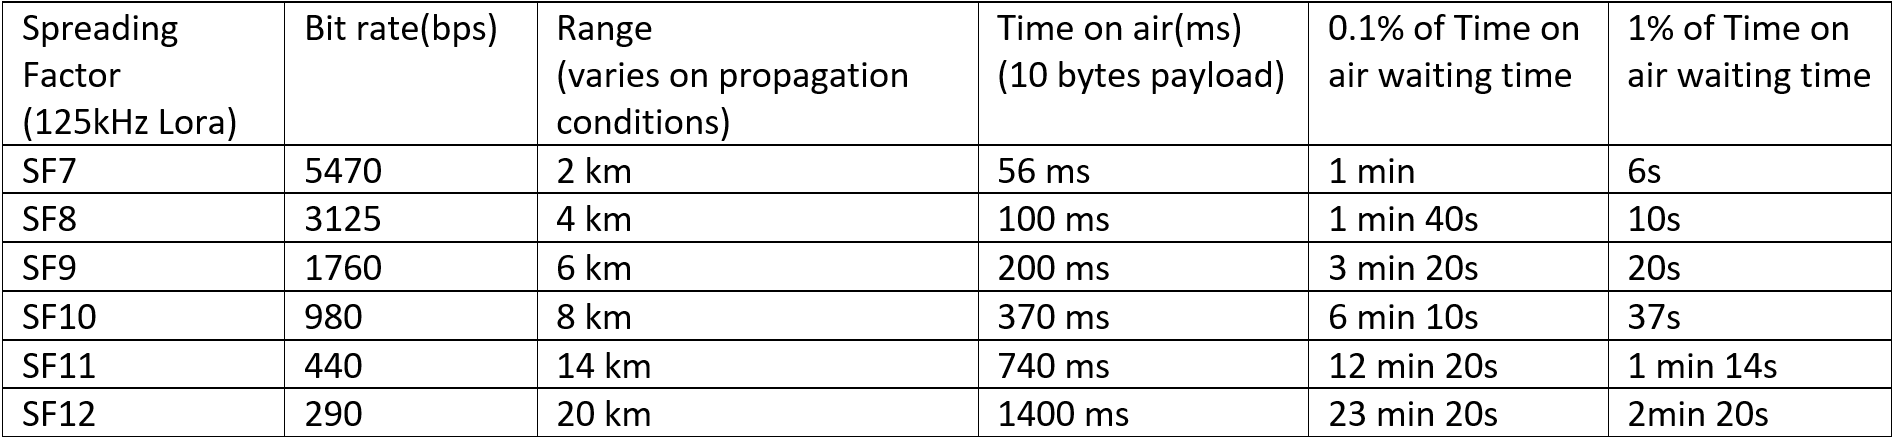
\includegraphics[width=1\textwidth]{spreading_factor_lorawan_2017-07-29}
%     \caption{LoRa spread factor options \cite{24}}
%     \label{fig:loraSF}
% \end{figure}

% \cite{19} \cite{20} \cite{21} \cite{22} \cite{23} \cite{24}.

\subsection{Zigbee}
Zigbee je specifikace navržena pro IoT aplikace, založena na standardu  IEEE 802.15.4, vyvinuta Zigbee alliancí \cite{Zigbee_alliance_about}.
Technologii Zigbee podporuje topologie mesh a hvězdice, většinou je použita topologie mesh pro rozšíření dosahu sítě, který je mezi dvěma zařízeními do 300 m na přímou viditelnost a 75 až 100 m v budově \cite{Zigbee_alliance_solution}. Jedna síť může obsahovat až 65000 zařízení.
Dostupné transceivery na trhu se pohybují okolo \$8–30 od více různých výrobců, taktéž je i na trhu dostupných mnoho Zigbee koncových zařízení.


\subsection{BLE}
BLE (Bluetooth Low Energy) je verze Bluetooth navržena pro minimální spotřebu energie, podporující topologie point-to-point, broadcast a mesh \cite{BT_alliance}.
Dosah mezi dvěma zařízeními je až 100 m \cite{BT_nordic}.
Dostupné transceivery na trhu se pohybují okolo \$5–20 od více různých výrobců. Stejně tak je i na trhu mnoho dostupných koncových zařízení, ale mnohdy jsou tato koncová zařízení kompatibilní pouze se zařízení v rámci jednoho výrobce, tudíž může být problém je implementovat do vlastní senzorové sítě. 



% \subsection{Z-Wawe}
% Z-Wave is intended for wireless connectivity for all possible smart home products, controlled by PC, phone, voice, etc. It's based on mesh network topology so every non-battery powered device works as a router to enhance the network range so the more devices are connected in one network, the stronger the network is \cite{27} \cite{28}.
% \subsection{Thread}
% This technology based on IPv6 was developed for home network controlled by smartphone, tablet or PC \cite{29} \cite{30} \cite{31}.


% \section{Shrnutí vlastností vybraných technologií}
% V tabulce \ref{table:shrnutiTechnologii} jsou shrnuty vlastnosti zmíněných technologií.   

\newpage

\section{Vybraná přenosová technologie}
% Tabulka \ref{table:shrnutiTechnologii} shrnuje vlastnosti zmíněných technologií.   

\begin{longtable}{|p{1.5cm}||p{1.3cm}|p{1.5cm}|p{1.4cm}|p{1.5cm}|p{2.8cm}|}
    \caption{Souhrn porovnání parametrů kandidátní bezdrátových technologií}
    \label{table:shrnutiTechnologii} \\ 
    \hline
 & \textbf{IQRF}         & \textbf{Wireless M-bus} & \textbf{LoRa}                 & \textbf{ZigBee}                          & \textbf{BLE}                                              \\ \hline \hline
    Topologie               & mesh, star            & star                  & star                            & mesh, star                               & Point-to-Point, Broadcast, Mesh                           \\ \hline
    Max. velikost paketu & 64 B                  & 256 B                 & 256 B                           & 133 B                                    & 20 B (Bluetooth 4.0), 251 B (Bluetooth 4.2)               \\ \hline
    Přenosová rychlost              & 19.2 kb/s             & 32.768 – 100 kb/s     & 0.3-50kb/s                      & 250 kb/s                                 & až 1 Mb/s                                              \\ \hline
    Pásmo (Evropa)          & 868 MHz               & 868 MHz               & 868 MHz                         & 2.4 GHz                                  & 2.4 GHz                                                   \\ \hline
    Dosah                  & 500 m (line of sight) & 500 m (line of sight) & 15-22 km suburban, 3-8 km urban & 300 m (line of sight), 75-100 m (indoor) & 100 m (class 1), 10 m (class 2), less then 10 m (class 3) \\ \hline
    Zabezp.               & AES128               & AES128               & AES128                         & AES128                                  & AES128                                                   \\ \hline
    Max. vysílací výkon & až 8 mW            & 0.16–20 mW            & 24 mW                           & 1-100 mW                                 & 100 mW (class 1), 5 mW (class 2), 1 mW (class 3)          \\ \hline

\end{longtable}

% Mezi hlavní kritéria pro vybranou bezdrátovou technologii patří nízká spotřeba energie koncových zařízení, nízká cena, jednoduchost implementace a možnost připojení koncových zařízení třetích stran.
% Všechny zmíněné kandidátní technologie jsou navrženy pro zařízení napájena z baterie a umožňují dlouhodobou životnost koncových zařízení napájených z baterie.

Technologie IQRF byla zavrhnuta, jelikož je na trhu velmi málo dostupných koncových zařízení třetích stran, které by bylo možné do sítě připojit. 
ZigBee a BLE mají příliš krátký dosah, což by bylo možné vyřešit rozmístěním více gatewayí napojených na přístupový systém nebo použitím mesh topologie, ale zvyšuje to složitost instalace a cenu řešení. 
Wireless M-bus a LoRa mají jako nevýhodu vysokou cenu transceiveru pro gateway. 
LoRa má možnost použití v jednokanálovém módu, kde gateway může použít transceiver určen pro koncová zařízení, který je víc jak desetkrát levnější a vyžaduje nižší výkon CPU (Central Processing Unit) než transceiver pro gateway, tudíž gateway v jednokanálovém módu je mnohem jednodušší a levnější řešení.
\\
Vzhledem k definovaným kritériím tedy byla vybrána techologie LoRa se standardizovaným síťovým protokolem LoRaWAN v jednokanálovém módu, jako je to používáno ve vývojových projektech \cite{Analysis of Propagation Link for Remote Weather}, tudíž to není plně LoRaWAN kompatibilní.
V jednokanálovém módu jsou všechna zařízení v síti nakonfigurována na jeden konkrétní kanál a SF.
LoRaWAN koncová zařízení třetích stran jsou plně kompatibilní s jakoukoliv LoRaWAN gatewayí pro daný region, tudíž mohou být implementovány do navrženého systému v tomto projektu, ale musí být překonfigurována ke komunikaci na zvoleném kanále a přenosové rychlosti. 
LoRaWAN síť má hvězdicovou topologii při dostatečném dosahu pro pokrytí budovy a jejím okolí, navíc dosah lze ladit parametrem SF. Pro tento vybraný případ senzorové sítě je to vhodné, jelikož pravděpodobně všechna zařízení v síti budou senzory napájeny z baterie, a není předpokládáno, že by byly připojeny zařízení umožňující směrování paketů z důvodu spotřeby energie. 
LoRaWAN síť umožňuje koncovým zařízením po změření dat senzory je ihned odeslat na gateway bez nutností čekání na potvrzení, tudíž se koncové zařízení může ihned přepnout do režimu spánku a tím eliminovat spotřebu energie. 
Případné občasně kolize mají za důsledek selhání doručení paketu, ale pro vybraný případ měřícího systému to není příliš závažný problém.
Frekvenční ISM pásmo 868 MHz, které používá LoRa je limitováno na maximální dobu vysílání 1\% času jedním zařízením a přenosová rychlost této technologie patři mezi nejnižší z kandidátních technologií. 
Pro vybraný případ měřícího systému se předpokládá přenášení pouhých hodnot senzorů o velikosti několik jednotek až desítek bytů s intervalem několika minut až hodin.
LoRaWAN protokol je zabezpečen šifrováním AES-128 na dva způsoby, a to zabezpečení aplikační pro nečitelnost přenášených dat a síťové pro zabránění útočníkům opakovat již přenesené pakety nebo odesílat falešné pakety, tudíž je toto zabezpečení dostatečné. 

% tahle section by mozna mohla byt nekde jinde
% \subsection{Zabezpečení protokolu LoRaWAN}
% Protokol LoRaWAN používá AES-128 na 2 způsoby, pro síťové a aplikační zabezpečení. Jsou zde tedy 2 šifrovací klíče, NwkSKey a AppSKey.

% \subsubsection{Síťové zabezpečení}
% Síťové zabezpečení je zde aby bylo hackerům zabráněno odesílání duplikovaných paketů nebo vytváření a vysílání paketů s nasimulovanými daty.
% Poslední 4 byty paketu obsahují MIC (Message Integrity Code), který je získán zašifrováním dat síťovým klíčem NwkSKey obsahujících mimo jiné celý payload paketu (včetně paket counter). Toto umožňuje odhalit jakoukoliv manipulaci s daty v paketu. LoRaWAN paket také obsahuje counter počítající od nuly od doby kdy bylo LoRaWAN zařízení spuštěno. Toto umožňuje odhalit duplikování paketů.

% \subsubsection{Aplikační zabezpečení}
% Aplikační klíč AppSKey (Application Session Key) je použit pro zašifrování dat aplikační zprávy (App message) \cite{lwSpec} \cite{lwSecur}.
